% \chapter{Results}
% \label{chapter:results}

%%% SECTION
\section{Introduction}
The following section summarizes the results obtained from running GSEA on the selected genes from the pipeline of the scenario 2.

\section{GSEA Results}
\subsection{Dataset Details}
The dataset has 183 native features.
After collapsing features into gene symbols, there are: 172 genes.

\subsection{Gene Set Details}
Gene set size filters (min=1, max=500) resulted in filtering out 61 / 189 gene sets.
The remaining 128 gene sets were used in the analysis.

\subsection{Enrichment in Positive Correlation}
\textbf{Enrichment in phenotype:} positive correlation with profile.
\begin{itemize}
\item 95 / 128 gene sets are upregulated in phenotype \textbf{208712\_at\_pos}.
\item 0 gene sets are significant at FDR minor than 25\%.
\item 0 gene sets are significantly enriched at nominal pvalue minor than 1\%.
\item 4 gene sets are significantly enriched at nominal pvalue minor than 5\%.
\end{itemize}

\subsection{Enrichment in Negative Correlation}
\textbf{Enrichment in phenotype:} negative correlation with profile.
\begin{itemize}
\item 33 / 128 gene sets are upregulated in phenotype \textbf{208712\_at\_neg}.
\item 0 gene sets are significantly enriched at FDR minor than 25\%.
\item 1 gene sets are significantly enriched at nominal pvalue minor than 1\%.
\item 2 gene sets are significantly enriched at nominal pvalue minor than 5\%.

\end{itemize}

\subsection{Gene List Correlation and Heatmap}

\begin{figure}[h]
    \centering
    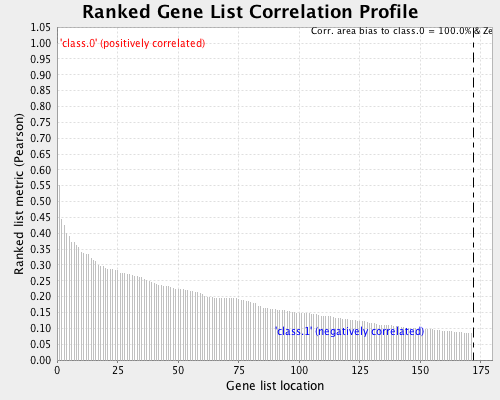
\includegraphics[scale=0.75]{../figs/ranked_list_corr_193.png}
    \caption{Ranked list correlations}
    \label{fig:gene-cor-1}
\end{figure}

\begin{figure}[h]
    \centering
    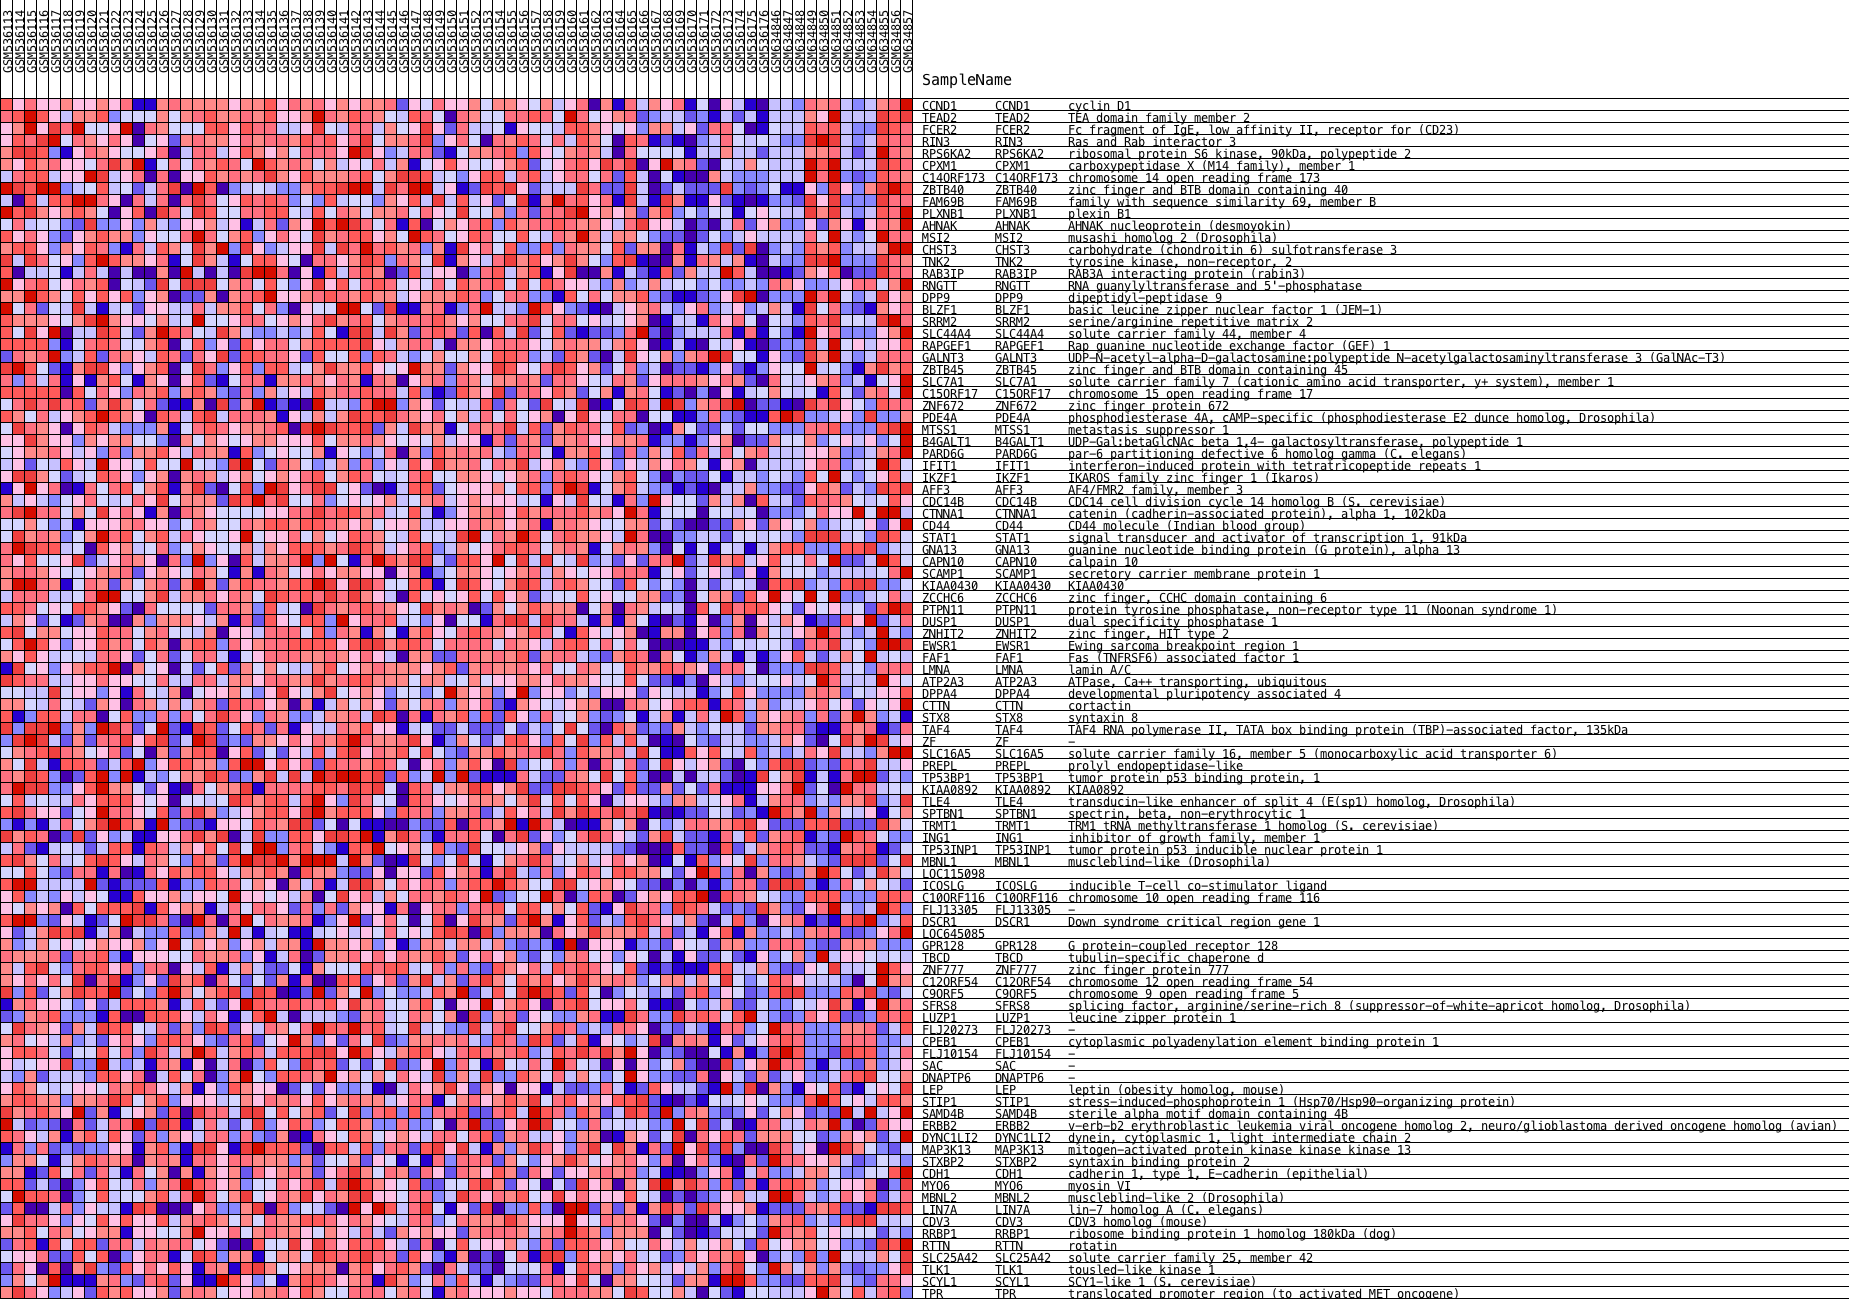
\includegraphics[width=\paperwidth]{../figs/heat_map_192.png}
    \caption{Heat Map of the top 50 features for each phenotype}
    \label{fig:heatmap-1}
\end{figure}
